% !TeX root = main.tex
\clearpage
\begingroup
\setlength{\emergencystretch}{3em}
\subsection{A3: Contratos de API y de Eventos}
\label{sec:fase5-a3}

Se definieron los contratos HTTP de los cuatro servicios de dominio y del
adaptador de Webhooks, junto con el catálogo de eventos de integración.
Los documentos se conservan en \path{cna/contracts/}. Las especificaciones
fijan las entradas, salidas, errores, correlación y compatibilidad que
implementarán los servicios de la Fase 6.

\subsubsection{Contratos HTTP en OpenAPI 3.1}
Los cinco documentos utilizan \texttt{openapi: 3.1.0}, esquemas de datos,
parámetros, ejemplos, seguridad y respuestas tipadas. La
Tabla~\ref{tab:f5-a3-http} resume las rutas de negocio. Los cuatro servicios
de dominio usan el servidor externo \path{https://api.bookstack.local}.
El adaptador opera exclusivamente en la red privada.

\begin{table}[H]
\centering\small
\begin{tabularx}{\textwidth}{p{2.9cm}XX}
\toprule
\textbf{Documento} & \textbf{Operaciones principales} & \textbf{Resultado} \\
\midrule
\path{search-svc.openapi.yaml} & GET \path{/v2/search?q=} & Libros y páginas con puntaje, resaltado y enlace al monolito. \\
\path{audit-svc.openapi.yaml} & GET \path{/v2/audit}; GET por \path{event_id} & Actividad filtrada por entidad, ID y rango temporal; consulta individual de evento. \\
\path{export-svc.openapi.yaml} & POST \path{/v2/exports}; GET por \path{job_id} & Aceptación 202, consulta de estados y archivo con URL prefirmada temporal. \\
\path{media-svc.openapi.yaml} & POST \path{/v2/media}; GET de metadatos, original y miniatura & Imagen persistida, miniatura proporcional y evento de subida. \\
\path{event-bridge.openapi.yaml} & POST \path{/internal/webhooks/bookstack} & Entrada autenticada, deduplicación y aceptación durable del Webhook. \\
\bottomrule
\end{tabularx}
\caption{Contratos HTTP de A3 y rutas principales.}
\label{tab:f5-a3-http}
\end{table}

Cada servicio expone además \path{/healthz}, \path{/readyz} y
\path{/metrics} mediante servidores internos por operación. La sonda de
vida verifica el proceso; la de disponibilidad comprueba las dependencias
necesarias para aceptar trabajo. Las métricas incluyen solicitudes por
código y un histograma de duración en formato Prometheus.

Las respuestas \textbf{200} entregan resultados disponibles y
\textbf{202} aceptan operaciones asíncronas. \textbf{400} identifica una
entrada inválida, \textbf{404} un recurso inexistente o fuera del alcance
visible, y \textbf{503} una indisponibilidad. Una búsqueda sin coincidencias
devuelve 200 con una lista vacía. Los errores comparten el esquema
\texttt{Error}, con código, mensaje y \path{request_id}. Se documentan
también 401/403 para autorización, 409 para conflicto de idempotencia,
413/415 para subidas y 429 para rate limiting.

La exportación admite exactamente un origen, página o libro, y formato PDF
o Markdown. El trabajo recorre \texttt{queued}, \texttt{running},
\texttt{done} o \texttt{failed}. El esquema de \texttt{done} exige el archivo
y su vencimiento; \texttt{failed} exige una causa. La clave
\path{Idempotency-Key} permite reconocer una solicitud repetida y rechaza
su reutilización con un contenido distinto.

Medios acepta PNG, JPEG y WebP, con límite inicial de 10 MiB y 20 millones
de píxeles. La miniatura conserva proporción y se limita a 320 por 320
píxeles. Estas restricciones forman parte del contrato de esta versión.

Las rutas externas requieren una credencial de consumidor
\path{X-API-Key}, administrada como secreto y separada del token interno
de BookStack. El servicio debe validar el alcance de acceso antes de
entregar texto, auditoría o archivos. La implementación inicial del
laboratorio se limita al contenido compartido autorizado para la cuenta
de servicio y sus consumidores. La autorización diferenciada por usuario
requiere proyectar o consultar sus permisos antes de ampliar ese alcance.

\subsubsection{AsyncAPI 3.0 y sobre de evento común}
El archivo \path{bookstack.asyncapi.yaml} utiliza
\texttt{asyncapi: 3.0.0}. Cada canal define su mensaje, el esquema del
payload, un ejemplo y las operaciones de envío y recepción identificadas
por componente. Los consumidores de páginas de búsqueda y auditoría son
durables e independientes, con confirmación explícita.

\begin{table}[H]
\centering\small
\begin{tabularx}{\textwidth}{p{5cm}XX}
\toprule
\textbf{Canal} & \textbf{Productor} & \textbf{Consumidores} \\
\midrule
\path{bookstack.page.created} & event-bridge & Búsqueda y auditoría \\
\path{bookstack.page.updated} & event-bridge & Búsqueda y auditoría \\
\path{bookstack.page.deleted} & event-bridge & Búsqueda y auditoría \\
\path{export.requested} & API/outbox de exportación & Auditoría \\
\path{export.completed} & Worker/outbox de exportación & Auditoría \\
\path{media.uploaded} & Medios & Auditoría \\
\bottomrule
\end{tabularx}
\caption{Los seis canales de integración requeridos por A3.}
\label{tab:f5-a3-canales}
\end{table}

El sobre común exige \path{event_id} de tipo UUID, \texttt{type},
\texttt{version}, \path{occurred_at} en ISO 8601 con zona,
\path{request_id} y \texttt{payload}. Se incorpora \texttt{traceparent}
opcional para la instrumentación de trazas. El tipo del evento es constante
para cada mensaje, y los payloads definen actor, entidad y datos propios
del hecho. Una exportación completada publica la clave durable del objeto;
la URL prefirmada temporal se obtiene por HTTP.

El siguiente ejemplo ilustra el contrato de actualización de página.
\begin{lstlisting}[basicstyle=\ttfamily\footnotesize,breaklines=true,columns=fullflexible,frame=single]
{
  "event_id": "4e07d48d-e610-4b7f-9d2c-a10e960ec8b7",
  "type": "bookstack.page.updated",
  "version": "1.0",
  "occurred_at": "2026-11-11T14:00:00Z",
  "request_id": "9c7059e1b4954ed8934ba05643761378",
  "payload": {
    "page_id": 42,
    "book_id": 7,
    "actor": {"id": 3, "name": "Usuario de laboratorio"},
    "source_revision": 2
  }
}
\end{lstlisting}

Los jobs ejecutables se reservan en Redis. El evento
\path{export.requested} describe el hecho para otros consumidores y evita
duplicar la ejecución del mismo trabajo en otra cola. La persistencia del
job y de su publicación pendiente debe ser atómica. La deduplicación y el
tratamiento de fallos siguen ADR-010.

\subsubsection{Adaptación del Webhook y aceptación durable}
El formato de entrada se contrastó con \texttt{WebhookFormatter} de la
instalación relevada. El puente convierte \texttt{page\_create},
\texttt{page\_update} y \texttt{page\_delete} a los tres tipos normalizados.
Obtiene el actor de \path{triggered_by}, el momento de \path{triggered_at}
y el ID de página de \path{related_item.id}. Tolera los campos adicionales
de BookStack y copia solo los definidos por su contrato.

El token compartido en query se valida antes de persistir y su valor se
redacta en los logs del puente y proxy. El código relevado de
\texttt{DispatchWebhookJob} registra fallos HTTP o de conexión sin
programar un nuevo intento de esa llamada. Por ello se refinan ADR-007 y
ADR-009 para que el puente guarde inbox y outbox en una transacción de
\texttt{bridge\_db} antes de responder 202. El publicador confirma
JetStream antes de marcar el outbox como enviado. La caída temporal del
broker permite recuperar la publicación desde esa entrada persistida.

Una repetición idéntica del Webhook conserva el UUID normalizado y recibe
200. La huella del JSON canónico de entrada se conserva durante al menos
siete días. La falta de identificador único de origen impide distinguir
dos acciones diferentes con cuerpos idénticos; ese límite se comprobará
con los eventos y revisiones reales durante la implementación.

El gateway inicia \path{X-Request-ID} y los servicios lo propagan a las
respuestas, llamadas, logs y eventos. El Webhook relevado no incorpora por
sí mismo el identificador de la edición original. El puente genera uno
cuando está ausente. La instrumentación del envío desde BookStack deberá
propagar el contexto para completar la prueba de trazas de extremo a
extremo. La recuperación del índice por API complementa los Webhooks;
recuperar toda la auditoría de entradas que nunca llegaron al puente
requiere un procedimiento específico de origen.

\subsubsection{Política de versionado y compatibilidad}
La versión de la ruta HTTP es independiente de la versión del esquema de
evento y de la revisión del documento de contrato.
\begin{enumerate}[leftmargin=1.5em,itemsep=4pt]
\item La API utiliza \path{/v2/}, con revisión documental
\texttt{info.version: 1.0.0}. Un cambio incompatible crea \path{/v3/} y
mantiene ambas rutas durante la migración, conservando el contrato de v2
para los consumidores existentes.
\item Los seis subjects actuales conservan mensajes con
\texttt{version: 1.0}. Los esquemas de sobre y payload son estrictos, por
lo que agregar campos requiere una evolución planificada del esquema.
\item Una versión incompatible de evento se publica en subjects separados,
por ejemplo \path{v2.bookstack.page.updated}, con
\texttt{version: 2.0}. Los consumidores antiguos mantienen sus subjects y
los nuevos reciben la representación compatible con su contrato.
\item Durante la transición se pueden publicar ambas representaciones del
mismo hecho, conservando el ID lógico y la correlación. Cada proyección
deduplica en su propio almacén y solo consume la versión para la que fue
diseñada.
\end{enumerate}

\subsubsection{F5-E4: Validación de especificaciones y ejemplos}
\label{sec:f5-a3-validacion}
La validación reproducible se ejecutó desde el directorio de contratos
mediante \path{node validate.mjs}. Las dependencias se fijan con
\path{pnpm-lock.yaml}; su instalación se verificó mediante
\path{pnpm install --frozen-lockfile --ignore-scripts}. El procedimiento
completo está en \path{cna/contracts/README.md}.

Spectral 6.17.1 valida los cinco OpenAPI; el parser oficial AsyncAPI 3.6.6
valida el catálogo de eventos. AJV 8.20.0 contrasta los ejemplos con los
esquemas. La ejecución final comprobó \textbf{242 ejemplos},
\textbf{9 rechazos esperados de entradas inválidas} y
\textbf{0 errores}. Las entradas negativas incluyen orígenes de
exportación ambiguos, trabajos terminados sin archivo, UUID inválido,
correlación ausente y versiones incompatibles.

El parser emite una recomendación informativa para adoptar AsyncAPI 3.1.
Se mantiene 3.0 por la consigna docente. La ejecución registra cero errores
y cero advertencias. Los resultados completos, versiones de herramientas,
usuario, hostname y hashes SHA-256 se guardan en
\path{cna/docs/evidencias/fase5/a3/validation-report.json} y
\path{cna/docs/evidencias/fase5/a3/validation-summary.txt}.

\begin{table}[H]
\centering\small
\begin{tabularx}{\textwidth}{p{1.4cm}p{1.9cm}X}
\toprule
\textbf{Prueba} & \textbf{Evidencia} & \textbf{Resultado} \\
\midrule
P29 & F5-E4 & Cinco OpenAPI 3.1 y un AsyncAPI 3.0 validados; seis canales, sobre común y política de versionado documentados; ejemplos y rechazos comprobados. Resultado PASS. \\
\bottomrule
\end{tabularx}
\caption{Validación de los contratos de A3 y continuación de la matriz de pruebas.}
\label{tab:f5-a3-prueba}
\end{table}

\IfFileExists{../../../cna/docs/evidencias/fase5/F5-E4-validacion-contratos.png}{%
\begin{figure}[H]
\centering
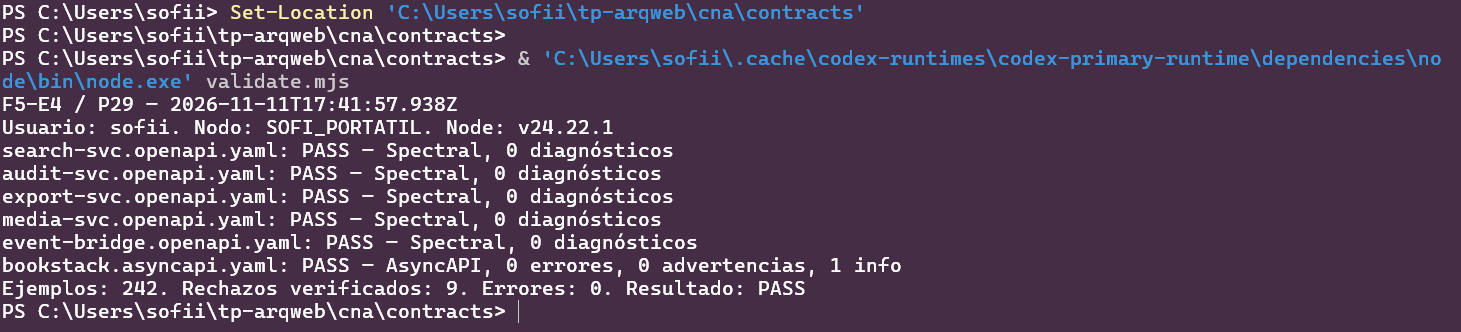
\includegraphics[width=\textwidth,height=0.6\textheight,keepaspectratio]{../../../cna/docs/evidencias/fase5/F5-E4-validacion-contratos.png}
\caption{F5-E4. Ejecución de los validadores de contratos con identificación del equipo y resultado final.}
\label{fig:f5-e4-validacion}
\end{figure}
}{}

Los contratos, el versionado y sus salidas de validación constituyen el
producto de diseño A3. La implementación de los endpoints, la durabilidad
del puente, el alcance de autorización y las interacciones se verificarán
en la Fase 6 conforme a estas especificaciones.
\endgroup
